\documentclass[t,12pt,numbers,fleqn,usenames,xcolor=dvipsnames]{beamer}
%\documentclass[t,12pt,numbers,fleqn,handout]{beamer}
% The theme: https://github.com/kailashbuki/beamerthemesaarland`

%\usetheme[
%background=saarland,
%logo=uds
%]{saarland}
%\graphicspath{{images/}}


\usepackage{amsmath}
\usepackage{mathtools}
\usepackage{amsfonts}
\usepackage{paralist}
\usepackage{latexsym}
\usepackage{amssymb}
\usepackage{stmaryrd}
\usepackage{phonetic}
\usepackage{wasysym}
\usepackage{pgf}
\usepackage{tikz}
\usepackage{url}
\usetikzlibrary{arrows}
\usepackage{array}
\usepackage{pgfpages} 
\usepackage{multirow} 
\usepackage{graphicx}
\usepackage{color}
\usepackage{listings,lstautogobble}
\lstset{
	basicstyle=\ttfamily,
	mathescape
}
\usepackage{hyperref}
\usepackage{verbatim}
\usepackage{fancyvrb}
\usepackage{tabularx}
\usepackage{tikz}
\usepackage{tikz-cd}
\usetikzlibrary{cd}
\usepackage{graphicx}
\usepackage{collectbox}
\usepackage{tabularx}
\usepackage{wrapfig}
\usepackage{lscape}
\usepackage{textcomp}

\usepackage[show]{ed}
\usepackage{smartdiagram}
\usesmartdiagramlibrary{additions}
\usepackage{adjustbox}
\setlength{\arrayrulewidth}{1mm}
\setlength{\tabcolsep}{18pt}
\renewcommand{\arraystretch}{1.5}
\hypersetup{colorlinks=false,
    linkcolor=blue,
    citecolor=blue,
    filecolor=blue,
    urlcolor=blue,
    unicode=false}

%\usepackage{macros}
%\usepackage{local}
%\usepackage{basics}

% To include lagda 
%\usepackage{latex/agda}
%\usepackage{ucs}
%\usepackage[utf8x]{inputenc}
%\usepackage{autofe}
%\usepackage{fancyvrb}
%\DefineVerbatimEnvironment
%{code}{Verbatim}


\lstset{language=lisp,basicstyle=\ttfamily,breaklines=true,showspaces=false,showstringspaces=false,breakatwhitespace=true,texcl=true,escapeinside={\%*}{*)}}
\tikzstyle{stuff_fill}=[rectangle,draw,fill=black!20,minimum size=1.4em]


\usepackage{fancybox}

\mode<presentation>{}


\usetheme{default}
\setbeamertemplate{navigation symbols}{} 
\setbeamertemplate{itemize item}[ball]
\setbeamersize{text margin left = 4mm}
\setbeamersize{text margin right = 4mm}

%\input{def-beamer}

\title{Leveraging Information in Theory Presentations}
\author{Yasmine Sharoda\\ \vspace{0.5cm} Supervisors: Jacques Carette and William Farmer}
\institute[]{Department of Computing and Software, McMaster University}
\date{July 8,2019}
	
\newcommand\textline[4][t]{%
	\par\smallskip\noindent\parbox[#1]{.333\textwidth}{\raggedright\texttt{+}#2}%
	\parbox[#1]{.333\textwidth}{\centering#3}%
	\parbox[#1]{.333\textwidth}{\raggedleft\texttt{#4}}\par\smallskip%
}	
\newcommand{\hilight}[1]{\colorbox{yellow}{#1}}
\setbeamertemplate{footline}[frame number]
	
\begin{document}

\begin{frame}
\titlepage
\end{frame}

\begin{comment}
\vfill
%\begin{center}
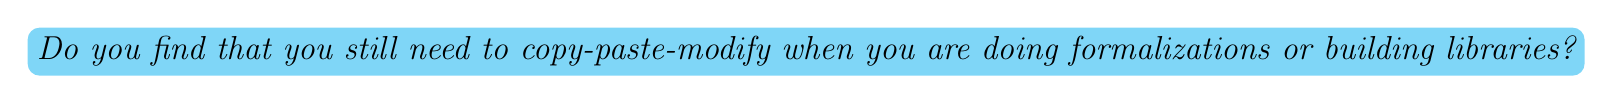
\begin{tikzpicture}
\node[preaction={fill=cyan,fill opacity=0.5},rounded corners=1ex,font=\fontsize{12pt}{12pt}\itshape] 
{Do you find that you still need to 
copy-paste-modify 
when you are doing formalizations or building libraries?};
\end{tikzpicture}
%\end{center}
\vfill
\end{comment}

\section{Motivation}
\begin{frame}[fragile]
\begin{tikzpicture}[overlay, remember picture]
\node[anchor=center] at (current page.center) {
	\begin{beamercolorbox}[center]{title}
Do you find yourself going through \\
\textbf{copy-paste-modify} flow?
	\end{beamercolorbox}};
\end{tikzpicture}

\end{frame}

\subsection{Agda Example}
\begin{frame}[fragile]
\frametitle{A Typical Task}
\begin{columns}
	\begin{column}{0.45\textwidth}
		\lstset{emph={} ,emphstyle=\fbox}
		\begin{lstlisting}[mathescape]
theory Foo { 
  U : type 
  s1 : U 
  $\hilight{s2 : U -> U -> U}$
}
		\end{lstlisting}
		\begin{lstlisting}
theory FooHom{
  f1 , f2 : Foo 
  h : f1.U $\rightarrow$ f2.U 
  pres-s1 : ... 
  pres-s2 : ... 
}
		\end{lstlisting}
	\end{column}
	\begin{column}{0.45\textwidth}
	 	\begin{lstlisting}
theory Bar {
  U : type 
  s1 : U 
  s2 : U $\rightarrow$ U 
}
	 	\end{lstlisting}
\pause
		\begin{lstlisting}
theory BarHom { 
  b1, b2 : Bar 
  h : b1.U $\rightarrow$ b2.U 
  pres-s1 : $\cdots$
  pres-s2 : $\cdots$
}
		\end{lstlisting}
	\end{column}
\end{columns}
\end{frame}

\begin{frame}[fragile]
\frametitle{A Typical Task}
\begin{columns}
\begin{column}{0.45\textwidth}
	\begin{lstlisting}
theory Foo { 
  U : type 
  s1 : U 
  s2 : U $\rightarrow$ U $\rightarrow$ U
} generates Hom 
	\end{lstlisting}
\end{column}
\begin{column}{0.45\textwidth}
	\begin{lstlisting}
theory Bar {
  U : type 
  s1 : U 
  s2 : U $\rightarrow$ U 
} generates Hom 
	\end{lstlisting}
\end{column}
\end{columns}
\end{frame}
%\frametitle{Example: Agda\footnote{code from: 
%\url{https://github.com/JacquesCarette/TheoriesAndDataStructures/}}}
%Define the category of group
%\begin{lstlisting}

%\end{lstlisting}
%\begin{columns}
%	\begin{column}{0.45\textwidth}
		
%		Agda monoid, TwoSorted, Pointed, AbelianGroup
%source: 
%https://github.com/JacquesCarette/TheoriesAndDataStructures/blob/master/Structures/TwoSorted.lagda
% \\
%source: 
%https://github.com/JacquesCarette/TheoriesAndDataStructures/blob/master/Structures/Pointed.lagda
% \\
%source: 
%https://github.com/JacquesCarette/TheoriesAndDataStructures/blob/master/Structures/AbelianGroup.lagda
%	\end{column}
%	\begin{column}{0.45\textwidth}
%       Agda Involutive
       %\footnote{source: 
       %\url{https://github.com/JacquesCarette/TheoriesAndDataStructures/blob/master/Structures/InvolutiveAlgebra.lagda}}
       %		
%	\end{column}
%\end{columns}


\begin{frame}
\frametitle{Real Example: Agda Library
\footnote{https://github.com/agda/agda-stdlib/blob/master/src/Algebra/Morphism.agda}}
Excerpts from the agda standard library (Semigroup and Monoid) 
\end{frame}

\subsection{Real Example: Isabelle Library}
\begin{frame}
\frametitle{Example: Isabelle \footnote{source: \url{https://isabelle.in.tum.de/dist/library/HOL/HOL-Algebra/index.html}}}
Show example from the Isabelle library (take it from the proposal)
\end{frame}

\subsection{Other Structures}
\begin{frame}
\frametitle{Other Structures?}
\vspace{0.15cm}
{\scriptsize
	Signature, Sub-algebra, Product-algebra, Projection of product algebra, Congruence-relation on 
	an algebra, Quotient algebra, Record definition of a theory, Homomorphism, 
	Homomorphism-equality, Composition of morphisms, Kernel of Homomorphism, Isomorphism, 
	Endomorphism, Automorphism, Closed term language, Open term language, Staged terms, 
	Structural induction, Evaluation function for terms, Simplification of terms, Rewrite rules, 
	Sub-terms of a term language, Equivalence of terms, Parse trees, Homomorphism between 
	terms and trees. 
}

\vspace{0.3cm}
\pause
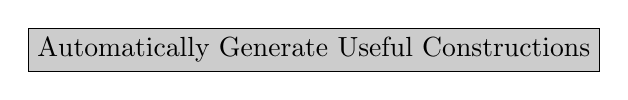
\begin{tikzpicture}
\draw (1, 1) node [stuff_fill] {Automatically Generate Useful Constructions};
\end{tikzpicture}
\
\end{frame}

\begin{frame}
\frametitle{Why is that Useful?}
Avoid Boilerplate 

boring, error-prone, counter productive and forgets the 
	mathematical structure
\end{frame}

\begin{frame}[fragile]
	\begin{center}
\smartdiagramset{
   uniform color list=white!60!black for 3 items, 
   back arrow disabled=true, 
   text width=2cm,
   additions={
      additional item offset=0.85cm,
      additional item border color=red,
	}
}
\smartdiagramadd[flow diagram:horizontal]{%
Abstract, Compute, Generate %
}{%
below of module1/Abstraction, below of module3/Specialization
}
	\end{center}
\end{frame}

\section{Algebraic Theories}
\begin{frame}
\frametitle{Algebraic Theories}
\begin{itemize}
	\item The examples we have seen all corresponds to algebraic theories. What is an algebraic theory?
	\item Abstractly, it has
	   \begin{itemize}
	   	\item sorts
	   	\item typed symbols: constants or functions 
	   	\item axioms 
	   \end{itemize}
   \item What do formal systems offer us? Show the slide about Monoid representations 
\end{itemize}
\end{frame}

\begin{frame}[fragile]
\frametitle{Monoid Theory}
\only<1>{
	\begin{figure}
		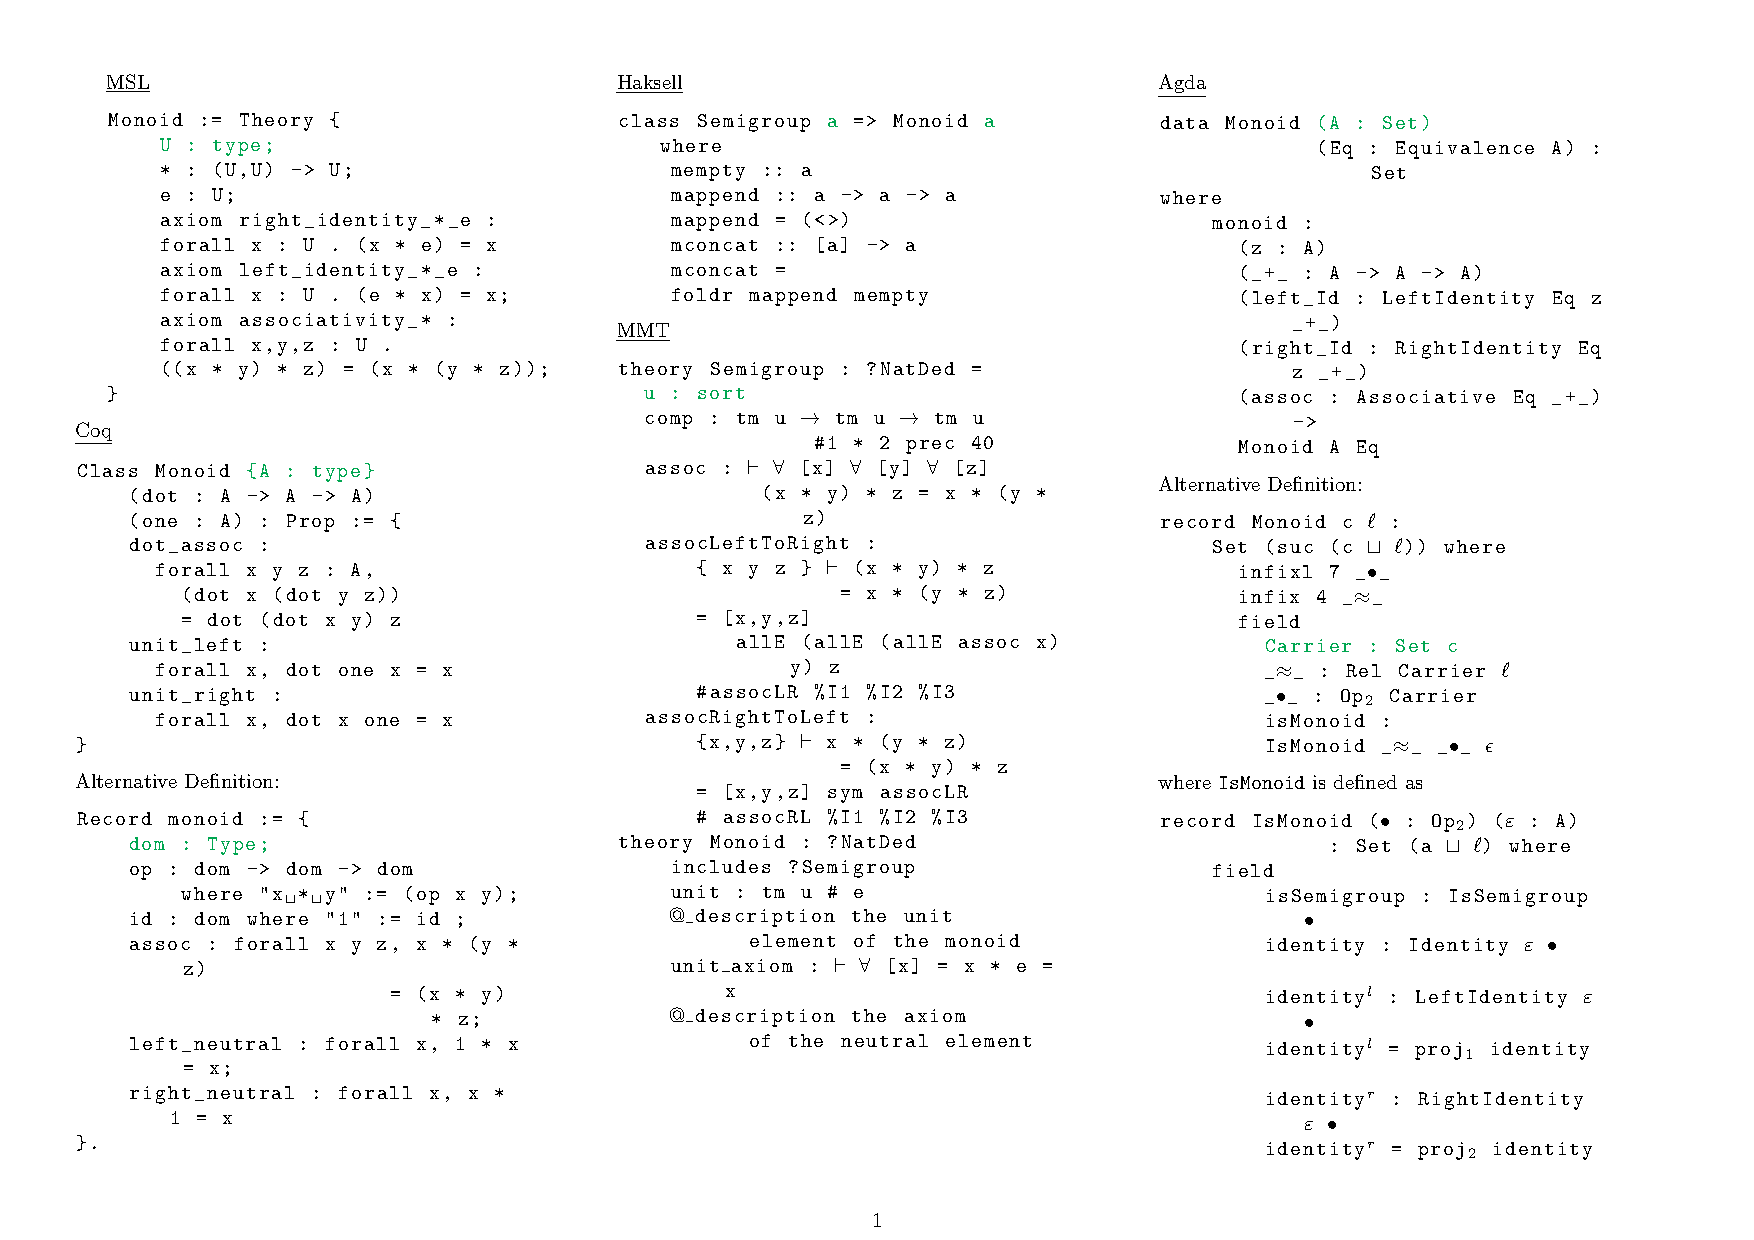
\includegraphics[scale=0.38]{monoid_highlighted.pdf}
	\end{figure}
}
\only<2>{
	\begin{tikzpicture}
	\draw (0, 0) node[inner sep=0] {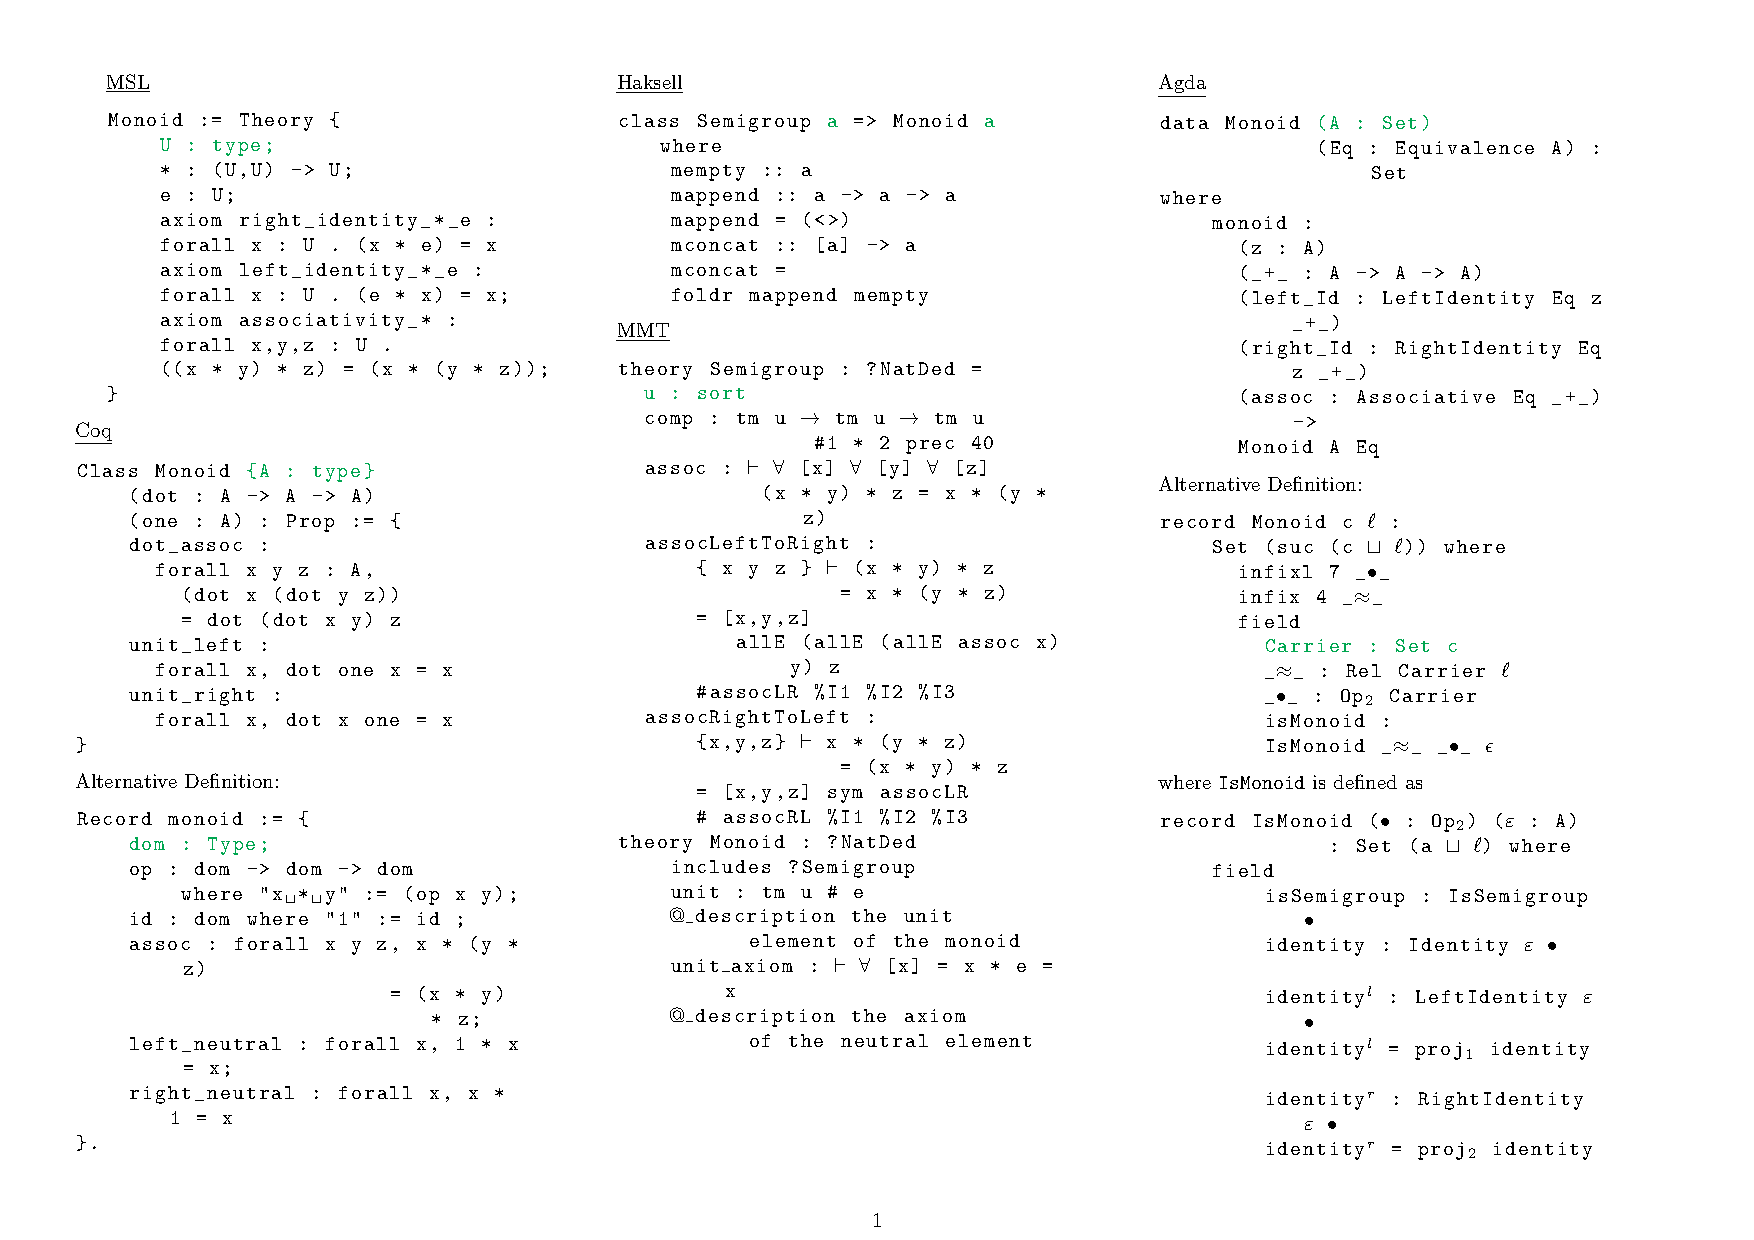
\includegraphics[scale=0.38]{monoid_highlighted.pdf}};
	\draw (0.5, 1) node [stuff_fill] {Abstract Over Details of Theory Presentations};
	\end{tikzpicture}
}
\end{frame}

\section{Research Objectives}
\begin{frame}
\frametitle{Research Objectives}
\begin{itemize}
	\item Generate Useful Algebraic Structures 
	\item Generate them in the most abstract setup 
	\item Translate the generated structures to various languages, 
	  \begin{itemize}
	  	\item Different Syntax
	  	\item Different Design Decisions
	  	\item Different Foundation 
	  	\item Example: Isabelle/HOL and Agda 
	  \end{itemize}
\end{itemize}
\end{frame}

\section{Approach}
\begin{frame}[fragile]
\frametitle{Abstraction: Use DDL}
	\begin{center}
\smartdiagramset{
			uniform color list=gray!60!black for 3 items,
			back arrow disabled=true,
			additions={
				additional item offset=0.85cm,
				additional item border color=red,
				additional connections disabled=false,
				additional arrow color=red,
				additional arrow tip=stealth,
				additional arrow line width=1pt,
				additional arrow style=]-latex’,
			}
}
\smartdiagramadd[flow diagram:horizontal]{%
PGF,Ti\textit{k}Z,Smartdiagram%
}{%
below of module1/Low Level, below of module3/High level%
}
\end{center}
\end{frame}

\begin{frame}
\frametitle{Use Feature Model to study formal systems}

\end{frame}

\begin{frame}
\frametitle{Use code generators to generate constructions in a specfic language}
\end{frame}

\section{Evaluation}
\begin{frame}
\frametitle{Evaluation: MathScheme Library}
Modularly constructed with 4 combinators 
capture the mathematical structure well enough 
\end{frame}

\section{Conclusion}
\begin{frame}
\frametitle{Conclusion}
A toolbox for building libraries that makes formalization tasks easier and leverages the information of the library 
\end{frame}

\end{document}



